%%% Класс документа
\documentclass[a4paper,14pt]{article}

%%% Работа с русским языком
\usepackage{cmap}					% поиск в PDF
\usepackage[warn]{mathtext}
\usepackage[T2A]{fontenc}			% кодировка
\usepackage[utf8]{inputenc}			% кодировка исходного текста
\usepackage[english,russian]{babel}	% локализация и переносы
\usepackage{mathtext} 				% русские буквы в формулах
\usepackage{csvsimple}              % for tabular from csv loading
\usepackage{indentfirst}            % indent after sections
%\usepackage{minipage}

%%% Дополнительная работа с математикой
\usepackage{amsmath,amsfonts,amssymb,amsthm,mathtools} % AMS
\usepackage{icomma} % "Умная" запятая: $0,2$ --- число, $0, 2$ --- перечисление

%%% Номера формул
%\mathtoolsset{showonlyrefs=true} % Показывать номера только у тех формул, на которые есть \eqref{} в тексте.
%\usepackage{leqno} % Немуреация формул слева

%%% Шрифты
\usepackage{euscript}	 % Шрифт Евклид
\usepackage{mathrsfs} % Красивый матшрифт

%%% Свои команды
\DeclareMathOperator{\sgn}{\mathop{sgn}}

%%% Перенос знаков в формулах (по Львовскому)
\newcommand*{\hm}[1]{#1\nobreak\discretionary{}
{\hbox{$\mathsurround=0pt #1$}}{}}

%%% Работа с картинками
\usepackage{graphicx}  % Для вставки рисунков
\graphicspath{{images/}{images2/}}  % папки с картинками
\setlength\fboxsep{3pt} % Отступ рамки \fbox{} от рисунка
\setlength\fboxrule{1pt} % Толщина линий рамки \fbox{}
\usepackage{wrapfig} % Обтекание рисунков и таблиц текстом

%%% Работа с таблицами
\usepackage{array,tabularx,tabulary,booktabs} % Дополнительная работа с таблицами
\usepackage{longtable}  % Длинные таблицы
\usepackage{multirow} % Слияние строк в таблице

%%% Теоремы
\theoremstyle{plain} % Это стиль по умолчанию, его можно не переопределять.
%\newtheorem{theorem}{Теорема}[section]
%\newtheorem{proposition}[theorem]{Утверждение}
 
%\theoremstyle{definition} % "Определение"
%\newtheorem{corollary}{Следствие}[theorem]
%\newtheorem{problem}{Задача}[section]
 
%\theoremstyle{remark} % "Примечание"
%\newtheorem*{nonum}{Решение}

%%% Программирование
\usepackage{etoolbox} % логические операторы

%%% Страница
\usepackage{extsizes} % Возможность сделать 14-й шрифт
\usepackage{geometry} % Простой способ задавать поля
	\geometry{top=25mm}
	\geometry{bottom=35mm}
	\geometry{left=35mm}
	\geometry{right=20mm}
	
%%% Колонтитулы
%\usepackage{fancyhdr}
 	%\pagestyle{fancy}
 	%\renewcommand{\headrulewidth}{0mm}  % Толщина линейки, отчеркивающей верхний колонтитул
 	%\lfoot{Нижний левый}
 	%\rfoot{Нижний правый}
 	%\rhead{Верхний правый}
 	%\chead{Верхний в центре}
 	%\lhead{Верхний левый}
 	% \cfoot{Нижний в центре} % По умолчанию здесь номер страницы
 	
%%% Интерлиньяж
%\usepackage{setspace}
%\onehalfspacing % Интерлиньяж 1.5
%\doublespacing % Интерлиньяж 2
%\singlespacing % Интерлиньяж 1

%%% Гиперссылки
\usepackage{hyperref}
\usepackage[usenames,dvipsnames,svgnames,table,rgb]{xcolor}
\hypersetup{				% Гиперссылки
    unicode=true,           % русские буквы в раздела PDF
    pdftitle={Заголовок},   % Заголовок
    pdfauthor={Автор},      % Автор
    pdfsubject={Тема},      % Тема
    pdfcreator={Создатель}, % Создатель
    pdfproducer={Производитель}, % Производитель
    pdfkeywords={keyword1} {key2} {key3}, % Ключевые слова
    colorlinks=true,       	% false: ссылки в рамках; true: цветные ссылки
    linkcolor=red,          % внутренние ссылки
    citecolor=green,        % на библиографию
    filecolor=magenta,      % на файлы
    urlcolor=cyan           % на URL
}

%%% Другие пакеты
\usepackage{lastpage} % Узнать, сколько всего страниц в документе.
\usepackage{soul} % Модификаторы начертания
\usepackage{csquotes} % Еще инструменты для ссылок
%\usepackage[style=authoryear,maxcitenames=2,backend=biber,sorting=nty]{biblatex}
\usepackage{multicol} % Несколько колонок
\usepackage{multirow} % Несколько строк

%%% Шрифты
%\renewcommand{\familydefault}{\sfdefault} % Начертание шрифта


%%% Работа с библиографией
%\usepackage{cite} % Работа с библиографией
%\usepackage[superscript]{cite} % Ссылки в верхних индексах
%\usepackage[nocompress]{cite} % 
%\usepackage{csquotes} % Еще инструменты для ссылок


%%% Tikz
\usepackage{tikz} % Работа с графикой
\usepackage{pgfplots} % Работа с pgf
\usepackage{pgfplotstable}
\usepackage{upgreek}

%%% Дополнительные пакеты для tikz
%\usepgfplotslibrary{dateplot} % Возможность подписания дат
\pgfplotsset{compat=1.5}

\begin{document}
    %\newcommand{\HRule}{\rule{\linewidth}{0.7mm}} % Defines a new command for the horizontal lines, change thickness here
	
	\begin{center}
		\large\textbf{Московский Физико-Технический Институт}\\ % Name of your university/college
		\large\textbf{(государственный университет)}
	
		\vfill
		
		\Large Лабораторная работа по курсу общей физики № *labnum*\\[0.5cm] % Preambule of your document title
		
		
		\HRule
		\\[0.4cm]
		{ \huge \bfseries *name of your labwork*}% Title of your document
		\\[0.4cm] 
		\HRule
		\\[0.5cm]
		
		\ \\
	\textbf{\large Автор:} \\	
	\large *your name* *groupname*\\ % Your name and something more, your group num for example
		\vfill
		\hspace*{-0.8 cm}
\includegraphics[width=100 pt]{frkt_logo}\\ % logo of your  company/university/college
		\large Долгопрудный, 2021 % location and year
	\end{center}

\newpage
\setcounter{page}{2}
\fancyfoot[c]{\thepage}
\fancyhead[L] {Работа № *labnum*} % some information in page header
\fancyhead[R]{}

    \noindent Проведем градуирование магнита.
    \begin{table}[h!]
    \begin{center}
        \begin{tabular}{|c|c|}
            \hline
            $B$, мТл & $I$, А \\ \hline
            1057     & 2,0   \\ \hline
            1032     & 1,8  \\ \hline
            978      & 1,6  \\ \hline
            935      & 1,4  \\ \hline
            845      & 1,2  \\ \hline
            730      & 1,0   \\ \hline
            611      & 0,8  \\ \hline
            491      & 0,6  \\ \hline
            338      & 0,4  \\ \hline
            \end{tabular}
    \end{center}
    \caption{}
\end{table}
    % график градуирования

    \noindent Измерим вольт-амперную характеристику образца.
    \begin{table}[h!]
    \begin{center}
        \begin{tabular}{|c|c|}
            \hline
            $I$, мА & $U$, мкВ \\ \hline
            0,2     & 361      \\ \hline
            0,3     & 530      \\ \hline
            0,4     & 703      \\ \hline
            0,5     & 875      \\ \hline
            0,6     & 1043     \\ \hline
            0,7     & 1220     \\ \hline
            0,8     & 1392     \\ \hline
            0,9     & 1565     \\ \hline
            1,0     & 1743     \\ \hline
        \end{tabular}
    \end{center}
    \caption{}
\end{table}
    
    \begin{figure}[h!]
        \centering
        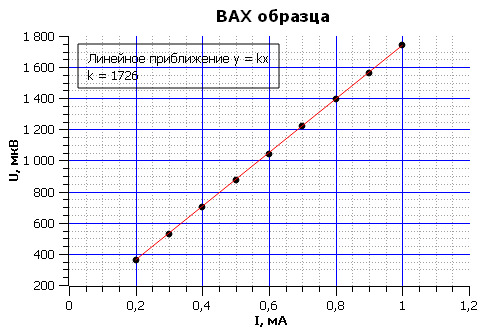
\includegraphics[scale = 1]{VAC.jpg}
        \caption{}
    \end{figure}

    \noindent Параметры образца.
    \begin{center}
        $a = 2,2$ мм -- ширина образца              \\
        $h = 2,5$ мм -- толщина образца             \\
        $L = 3,0$ мм -- расстояние между контактами \\
    \end{center}

    \noindent Удельное сопротивление образца можем посчитать по формуле
    \begin{equation*}
        \rho_0 = \frac{U_{35} a h}{I L}
    \end{equation*}
    \noindent Величину $\frac{U_{35}}{I}$ найдем из графика.

    \begin{center}
        \fbox{$\rho_0 = 0,312 ~ \text{Ом} \cdot \text{см}$}
    \end{center}

    \noindent Найдем отсюда удельную проводимость.

    \begin{center}
        \fbox{$\sigma = 3,2 ~ (\text{Ом} \cdot \text{см})^{-1}$}
    \end{center}

    \noindent Снимем зависимость ЭДС Холла от значения индукции магнитного поля при разных значениях продольного тока.
    Заметим, что напряжение на контактах связано не только с эффектом Холла, но и с 
    оммическим падением напряжения вдоль пластины. Исключить этот эффект можно двумя способами:

    \begin{enumerate}
        \item Изменять направление магнитного поля, пронизывающего образец. При обращении поля знак
        ЭДС Холла меняется, поэтому ЭДС Холла $U_{34}$ может быть определена по формуле
        \begin{equation*}
            U_{\bot} = \frac{U^{(+)} - U^{(-)}}{2}
        \end{equation*}
        \item Можно исключить влияние оммического падения напряжения, измеряя падение напряжения на образце $U_0$
        в отсутсвии магнитного поля. Тогда ЭДС Холла вычисляться по формуле
        \begin{equation*}
            U_{\bot} = U_{34} - U_0
        \end{equation*}
    \end{enumerate}

    \newpage
    % ------------------------------------------------------------------------------------------------------------------------
    \begin{center}
        $I = 1$    мА  \\
        $U_0 = -38$ мкВ \\
    \end{center}
    \begin{table}[h!]
    \begin{center}
        \begin{tabular}{|c|c|c|c|c|}
            \hline
            $U^{(+)}$, мкВ & $U^{(-)}$, мкВ & $U_{\bot}$, мкВ & $B$, мкТл & $I$, А \\ \hline
            166            & -237           & 202             & 1057      & 2,0    \\ \hline
            157            & -230           & 194             & 1032      & 1,8    \\ \hline
            149            & -221           & 184             & 978       & 1,6    \\ \hline
            137            & -210           & 174             & 935       & 1,4    \\ \hline
            121            & -193           & 157             & 845       & 1,2    \\ \hline
            99             & -172           & 136             & 730       & 1,0    \\ \hline
            75             & -148           & 112             & 611       & 0,8    \\ \hline
            49             & -122           & 86              & 491       & 0,6    \\ \hline
            23             & -95            & 59              & 338       & 0,4    \\ \hline
        \end{tabular}
    \end{center}
    \caption{}
\end{table}
    \begin{figure}[h!]
        \centering
        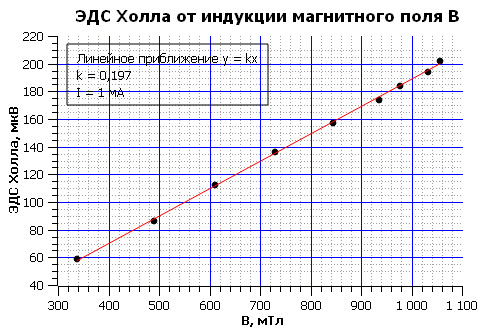
\includegraphics[scale = 1]{HallEffectI1.jpg}
        \caption{}
    \end{figure}
    % ------------------------------------------------------------------------------------------------------------------------
    \newpage
    \begin{center}
        $I = 0,5$    мА  \\
        $U_0 = -17$ мкВ \\
    \end{center}
    \begin{table}[h!]
    \begin{center}
        \begin{tabular}{|c|c|c|c|c|}
            \hline
            $U^{(+)}$, мкВ & $U^{(-)}$, мкВ & $U_{\bot}$, мкВ & $B$, мкТл & $I$, А \\ \hline
            52             & -72            & 62              & 1057      & 2      \\ \hline
            50             & -69            & 60              & 1032      & 1,8    \\ \hline
            47             & -66            & 57              & 978       & 1,6    \\ \hline
            44             & -63            & 54              & 935       & 1,4    \\ \hline
            39             & -58            & 49              & 845       & 1,2    \\ \hline
            32             & -52            & 42              & 730       & 1      \\ \hline
            25             & -44            & 35              & 611       & 0,8    \\ \hline
            17             & -36            & 27              & 491       & 0,6    \\ \hline
            8              & -28            & 18              & 338       & 0,4    \\ \hline
            \end{tabular}
    \end{center}
\end{table}
    \begin{figure}[h!]
        \centering
        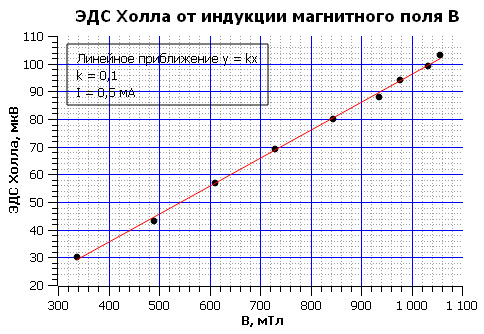
\includegraphics[scale = 1]{HallEffectI2.jpg}
        \caption{}
    \end{figure}
    % ------------------------------------------------------------------------------------------------------------------------
    \newpage
    \begin{center}
        $I = 0,3$    мА  \\
        $U_0 = -10$ мкВ \\
    \end{center}
    \begin{table}[h!]
    \begin{center}
        \begin{tabular}{|c|c|c|c|c|}
            \hline
            $U^{(+)}$, мкВ & $U^{(-)}$, мкВ & $U_{\bot}$, мкВ & $B$, мкТл & $I$, А \\ \hline
            85             & -120           & 103             & 1057      & 2      \\ \hline
            82             & -115           & 99              & 1032      & 1,8    \\ \hline
            77             & -110           & 94              & 978       & 1,6    \\ \hline
            71             & -105           & 88              & 935       & 1,4    \\ \hline
            63             & -96            & 80              & 845       & 1,2    \\ \hline
            52             & -85            & 69              & 730       & 1      \\ \hline
            40             & -73            & 57              & 611       & 0,8    \\ \hline
            26             & -60            & 43              & 491       & 0,6    \\ \hline
            13             & -47            & 30              & 338       & 0,4    \\ \hline
        \end{tabular}
    \end{center}
    \caption{}
\end{table}
    \begin{figure}[h!]
        \centering
        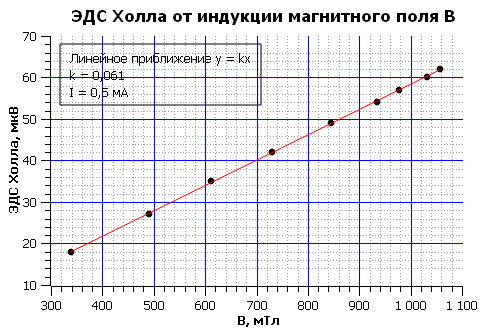
\includegraphics[scale = 1]{HallEffectI3.jpg}
        \caption{}
    \end{figure}
    % ------------------------------------------------------------------------------------------------------------------------
    \noindent По полученным данным вычислим концентрацию носителей зарядов в образце $n$.

    \begin{equation*}
        \varepsilon_h = \frac{I B}{n e a} = R_h \frac{I B}{a}
    \end{equation*}

    \noindent Найдем подвижность носителей зарядов $\mu$ в образце, спользуя формулу
    \begin{equation*}
        \sigma = e n \mu \Rightarrow \mu = \frac{\sigma}{e n}
    \end{equation*}

    \noindent где $e$ -- элементарный заряд, а $R_h = \frac{1}{n e}$ -- постоянная Холла. Тогда

    \begin{table}[h!]
    \begin{center}
        \begin{tabular}{|c|c|c|c|}
            \hline
            $I$  мА & $R_h \cdot 10^{-3}  ~ \frac{\text{Ом}}{\text{А}}$ & $n \cdot 10^{16} ~ \text{см}^{-3}$ & $\mu \cdot 10^3 ~ \frac{\text{см}^2}{\text{В} \cdot \text{с}}$  \\ \hline
            1,0     & 0,418                                             & 1,50                               & 1,33                                                            \\ \hline
            0,5     & 0,440                                             & 1,40                               & 1,43                                                            \\ \hline
            0,3     & 0,447                                             & 1,39                               & 1,44                                                            \\ \hline                
        \end{tabular}
    \end{center}
    \caption{}
\end{table}

\end{document}